% Authors: Simon Geoffroy-Gagnon and Farhad Shokraneh
% Based on the Thesis by Rubana Bahar Priti
% Edit: 2020.04.16

\documentclass[12pt, TexShade, letterpaper]{report}
\usepackage[utf8]{inputenc}
\usepackage{palatino}
\usepackage{amsmath}
\usepackage{amssymb}
\usepackage{graphicx}
\usepackage[labelfont=bf]{caption}
\usepackage{subcaption}
\usepackage{setspace}
\captionsetup[table]{font = {stretch=1.35}}
\captionsetup[figure]{font = {stretch=1.35}}
\usepackage[margin=1in, headsep=1cm, bottom=5cm]{geometry}
\usepackage[hidelinks]{hyperref}
\newcommand{\MYhref}[3][blue]{\href{#2}{\color{#1}{#3}}}%
\usepackage{tabu}
\usepackage{cite}
\usepackage[table]{xcolor}
\usepackage{nomencl}
\usepackage[nonumberlist,nogroupskip,xindy]{glossaries}
\usepackage{floatrow}
\usepackage{wrapfig}
\renewcommand{\baselinestretch}{2}
\usepackage{fancyhdr}
\usepackage{lmodern}
\usepackage{listings}

\renewcommand{\chaptermark}[1]{\markboth{#1}{}} % Ensure List of Figs, ToC, and glossary are named in the header

\setglossarystyle{long}
\renewcommand{\glsnamefont}[1]{\textbf{#1}}

\newglossarystyle{mystyle}{%
	\renewenvironment{theglossary}%
	{\begin{longtabu} to \linewidth {p{0.15\linewidth}p{0.85\linewidth}}}%
		{\end{longtabu}}%
	\renewcommand*{\glossaryheader}{}%
	% indicate what to do at the start of each logical group
	\renewcommand*{\glsgroupheading}{}
	\renewcommand*{\glsgroupskip}{}%
	\renewcommand*{\glossaryentryfield}[5]{%
		\glstarget{##1}{##2}% Name
		& ##3% Description
		\\% end of row
	}
}

% Overwrite the plain page style with a red line and page numbering
\fancypagestyle{plain}{%
	\fancyhf{} % clear all header and footer fields
	\fancyhead[R]{\textbf{\thepage}} % except the center
}

% Create the fancy page style header
\pagestyle{fancy}
\fancyhf{}
\lhead{\textbf{\nouppercase{\leftmark}}}
\chead{}
\rhead{\textbf{\thepage}}


\usepackage{xpatch}
\xpretocmd\headrule{\color{red}}{}{\PatchFailed}

% Get rid of all dashed words
\tolerance=1
\emergencystretch=\maxdimen
\hyphenpenalty=10000
\hbadness=10000

% Create glossary
\newacronym{lm}{LM}{Levenberg-Marquardt}
\newacronym{mcmc}{MCMC}{Markov Chain Monte Carlo}
\newacronym{dls}{DLS}{Damped Least-Squares}
\newacronym{ares}{ARES}{The Accelerated Reionization Era Simulations}
\newacronym{edges}{EDGES}{Experiment to Detect the Global EoR Signature}
\newacronym{eor}{EoR}{Epoch of Reionization}
\newacronym{igm}{IGM}{Intergalactic Medium}
\newacronym{sfr}{SFR}{Star Formation Rate}
\newacronym{saras}{SARAS}{The Shaped Antenna to measure the background Radio Spectrum}
\newacronym{cmb}{CMB}{Cosmic Microwave Background}
\makeindex
\makeglossaries

% Set page numbering to roman
\setcounter{page}{2}\renewcommand{\thepage}{\roman{page}}

\author{\textcopyright Author, August, 2020}
\date{}

\begin{document}

\begin{titlepage}
		\begin{center}
			\vspace*{0.5cm}

			\LARGE
			\textbf{Parameter Estimation of Global 21cm Signal}
			%Probing the Effect of Non-Standard Physics on Future 21cm Observations
			\vspace{1cm}
			
			\textit{Aryana Haghjoo}
			
			\vspace{1.2cm}
			
			
\includegraphics[width=0.25\textwidth]{mcglogo.png}
			
			\Large
			Department of Physics
			
			\vspace{-5mm}
			McGill University
			
			\vspace{-5mm}
			Montr\'eal, Qu\'ebec, Canada
			
			\vspace{5mm}
			August 2023
			\small
			\vspace{0.5cm}
			{\color{red} \hrule height 0.75mm}
			
			\vspace{0.2cm}
			
			A thesis presented for the degree of
			Masters of Physics
		
			\copyright\hspace{0.5mm}2023 Author
			
		\end{center}
	\end{titlepage}
\setlength{\voffset}{2cm}
\renewcommand{\chaptermark}[1]{%
	\markboth{\thechapter.\ #1}{}}
\chapter*{Abstract}\markboth{Abstract}{}
	\label{chap:engAbstract}
%	\addcontentsline{toc}{section}{\nameref{chap:engAbstract}}
The global 21cm signal has been used to study the period between the end of the cosmic dark ages and the formation of the first stars and galaxies. \par
In this study, we explore the potential of this signal to reveal non-standard physics by means of providing a new path to test fundamental physical theories. The 21cm signal is sensitive to the density and temperature of neutral hydrogen in the early universe and the presence of the first stars and galaxies. Therefore, any deviation from the predictions of the standard cosmological model of this signal could indicate the presence of new physics beyond the standard model.\par
We adopt the Markov Chain Monte Carlo (MCMC) method combined with the Levenberg Marquardt (LM) algorithm to estimate the best-fit physical parameters (e.g., clumping factor, star formation efficiency) of the theoretical 21cm curves. We use the Accelerated Reionization Era Simulations (ARES) to generate models for the global 21-cm signal. Our method is flexible to the choice of parameters from ARES.
The knowledge of these best-fit parameters will help us to constrain future proposed models and set theoretical limits for the precision of upcoming experiments to observe non-standard effects.\par

\chapter*{Abrégé}\markboth{Abrégé}{}
	\label{chap:frAbstract}
%	\addcontentsline{toc}{section}{\nameref{chap:frAbstract}}
Le signal global de 21 cm a été utilisé pour étudier la période entre la fin de l'âge sombre cosmique et la formation des premières étoiles et galaxies. \par
Dans cette étude, nous explorons le potentiel de ce signal pour révéler la physique non standard en fournissant une nouvelle voie pour tester les théories physiques fondamentales. Le signal de 21 cm est sensible à la densité et à la température de l'hydrogène neutre dans l'univers primordial et à la présence des premières étoiles et galaxies. Par conséquent, tout écart par rapport aux prédictions du modèle cosmologique standard de ce signal pourrait indiquer la présence d'une nouvelle physique au-delà du modèle standard.\par
Nous adoptons la méthode Markov Chain Monte Carlo (MCMC) combinée à l'algorithme de Levenberg Marquardt (LM) pour estimer les paramètres physiques les mieux adaptés (par exemple, facteur d'agrégation, efficacité de formation d'étoiles) des courbes théoriques de 21 cm. Nous utilisons les simulations d'ère de réionisation accélérée (ARES) pour générer des modèles pour le signal global de 21 cm. Notre méthode est flexible au choix des paramètres d'ARES.
La connaissance de ces paramètres de meilleur ajustement nous aidera à contraindre les futurs modèles proposés et à fixer des limites théoriques pour la précision des expériences à venir pour observer les effets non standard.\par
\chapter*{Acknowledgements}\markboth{Acknowledgements}{}
	\label{chap:acknowledgments}
%	\addcontentsline{toc}{section}{\nameref{chap:acknowledgments}}


Revised: 
I would like to express my gratitude to my supervisors, Jonathan Sievers and Oscar Hernandez, for their invaluable support throughout this project. I am also deeply grateful to my parents for their unwavering support, even from thousands of kilometers away. Additionally, I want to thank my new friends in Montreal for the wonderful experiences we shared.\par
Furthermore, I would like to acknowledge the significant role that my therapist at McGill Wellness Hub, Romeo Bidar, played in my graduate journey. His constant presence was a true blessing.\par
I must also mention the immense help that my two favorite Persian singers, Kamran and Hooman, provided through their Spotify playlist, which kept me motivated while debugging my code.\par
Lastly, I want to acknowledge my own perseverance and hard work, which enabled me to gain new experiences and insights.\par
 To all the lifelong learners and doers: you are changing the world every day.
 % Start of ToC, LoT, gls
	\tableofcontents\thispagestyle{plain}

	\listoffigures\thispagestyle{plain}
%	\addcontentsline{toc}{section}{\listfigurename}
	\listoftables
%	\addcontentsline{toc}{section}{\listtablename}
	\glsaddall
	\setlength\LTleft{0pt}
	\setlength\LTright{0pt}
	\setlength\glsdescwidth{0.8\hsize}
	\printglossary[title={List of Acronyms}]
	\markright{List of Acronyms} 

 	\clearpage
	\pagenumbering{arabic} % restart page numbers at one, now in arabic style
	
	\glsresetall
	% start of mainmatter
%###########################################################
\chapter{Introduction}
\label{chap:intro}
Reminder: The preface can be expanded, I should come back to writing this chapter after I am done with chapter 2 and 3. I guess it would help to have some addressing of those information here. \par
21cm cosmology in a relatively new opened window in the study of universe during its early states. It has been proven to be one of the only available probes of large-scale structure in the most distant reaches of the universe\cite{primordial_universe}.\par
In this chapter we will talk bout the importance of this signal and its applications. Then, we will describe the motivations of this research to clarify the effects non-standard physics on this signal. Although this signal can be studied in various forms (e.g. power spectrum, fluctuations, global signal, and etc.), we will only focus on the global 21cm signal.\par
Finally, in the last section of this chapter, we will briefly go over all the materials provided in this thesis.\par
%-----------------------------------------------------------
\section{Background and motivation}
Reminder: needs rephrasing\par
During the very early states of the universe, when there were not yet any galaxies or stars, the universe was composed of huge clouds of gas (mostly from hydrogen and helium) and the remaining photons from the big bang which we call cosmic microwave background (CMB). \par
Neutral hydrogen has a special spin-flip transition in its ground state which results in absorption or emission of a radio signal with the wavelength of 21cm. When the CMB photons redshift through time, there comes a period when they reach wavelengths of approximately 21cm. During this period, hydrogen molecules are able to absorb CMB photons (which we will later recall as coupling of $T_s$ with $T_k$). This process (which changes the brightness temperature of 21cm signal), happens roughly during the dark ages/epoch of reionization. This change in the brightness temperature ($T_b$) can be detected through precise observation using radio telescopes. These observations are capable of giving us valuable information about the distribution of neutral hydrogen and evolution of cosmic structure over time\cite{low_frequency}.\par
The global 21cm signal is the average over the brightness temperature of 21cm signal across the entire sky. It is a measure of overall state of intergalactic medium (IGM) which might present as absorption or emission during different redshits. Global 21cm signal can give us information about the temperature, density and reionization state of IGM in the early universe. These properties are determined by the complex interplay between the cosmic radiation field, the formation and evolution of the first stars and galaxies, and the feedback processes that these sources exert on their surroundings\cite{21century}.\par
Moreover, the global 21cm signal is a Strong probe for non-standard physics during the dark ages. It can show effects dark matter/dark energy, existence of cosmic strings, and etc. These effects will be discussed more in \ref{chap:global21cm,sub:non_standard}.\par
%-----------------------------------------------------------
\section{Research questions and objectives}
Reminder: citations, rephrasing \par
The effects of non-standard physics in 21cm signal has gained lots of attraction in the recent literature (cite). However, most of the reported effects has been investigated only using analytical methods, regardless of the observational data.\par
We aim to fill this research gap by probing these effects using semi-analytical simulations of the global 21cm signal. By having the recent released data in hand (cite edges) and comparing them to theoretical simulated data (cite ares), we first estimate the physical parameters of these models assuming only the standard physics. \par
In future studies, we will upgrade our simulator to include arbitrary non-standard effects. We will again fit our upgraded theoretical model to the observational data to check if any of the best-fit physical parameters show patterns of change.
%-----------------------------------------------------------
\section{Overview of the thesis}
Reminder: citations, rephrasing\par
This thesis consists of two major sections: the literature review and the research.\par
The literature review:\par
In chapter \ref{chap:global21cm}, we first talk about the global 21cm signal and the physical theory behind it. we will explain each bump in the plot. In section \ref{chap:global21cm,sub:non_standard}, we explore the effects of non-standard physics on global 21cm signal mentioned in the literature. Finally, in section \ref{chap:global21cm,sub:parameter_estimation}, we talk about the importance of estimating the parameters of this signal and how these estimations affects future proposed observations. Furthermore, we briefly talk about different methods used to serve this purpose and advantages of each one.\par
In chapter \ref{chap:observations} we will briefly introduce all of the past, present and future observational project who aim to detect the global 21cm signal. From all these experiments, we will specifically talk about two of them in detail.\par
The research:\par
In the research half of this thesis, we will talk about the parameter estimation of global 21cm signal. The specific method used in this this study is described in chapter \ref{chap:method} in detail. The results of using this method to fit the edges data are shown in chapter \ref{chap:results}. Finally, in chapter \ref{chap:discussion}, we talk interpret the results and talk the implications of these results for cosmology and astrophysics. Also, the limitations and the future prospective of the project is mentioned in this chapter.\par
%###########################################################
\chapter{The Global 21cm Signal}
\label{chap:global21cm}
%-----------------------------------------------------------
\section{Theoretical basis and physical principles of the Global 21cm Signal}
%-----------------------------------------------------------
\section{Simulating the global 21cm signal}
\subsection{The Accelerated Reionization Era Simulations (ARES)}
\subsection{21cmFast}
%------------------------------------------------------------
\section{Effects of non-standard physics on the global 21cm signal}
\label{chap:global21cm,sub:non_standard}
\subsection{Cosmic Strings}
\subsection{Dark Matter}
\subsection{Other non-standard effects}
\section{Parameter estimation of global 21cm signal}
\label{chap:global21cm,sub:parameter_estimation}
\subsection{Machine Learning}
\subsection{MCMC}
%##############################################################
\chapter{Observations of the Global 21cm Signal}
\label{chap:observations}
List of experiments (reminder: rephrasing and citing each of them,  things that I need for each experiment: dipole antenna, location, time frame of results, frequency range):\par
\begin{enumerate}
\item EDGES (Experiment to Detect the Global EoR Signature): This was the first experiment to report a detection of the global 21cm signal in 2018, by measuring the absorption of radio waves from distant sources by neutral hydrogen in the intergalactic medium.

\item SARAS (Small Array for Research in Astrophysics of the South): This is a radio telescope located in India that has been used to study the global 21cm signal since 2015.

\item SCI-HI (Small Radio Telescope for Cosmic Hydrogen Intensity Mapping): This is a low-frequency radio telescope located in the United States that was designed to detect the global 21cm signal during the epoch of reionization.

\item BIGHORNS (Broadband Instrument for Global HydrOgen ReioNisation Signal): This is a radio interferometer located in Australia that was designed to detect the global 21cm signal during the epoch of reionization.

\item HERA (Hydrogen Epoch of Reionization Array): This is a radio interferometer located in South Africa that is designed to detect the global 21cm signal during the epoch of reionization and cosmic dawn.

\item Tianlai: This is a radio interferometer located in China that is designed to detect the global 21cm signal during the epoch of reionization and cosmic dawn.

\item Murchison Widefield Array: This is a radio interferometer located in Australia that is used to study the early Universe, including the global 21cm signal.

\item LOFAR (Low-Frequency Array): This is a radio interferometer located in the Netherlands that is used to study a wide range of astrophysical phenomena, including the global 21cm signal.
\item PRIZM (Polarized Radiometer In Space) is another experiment designed to study the global 21cm signal. It is a small satellite mission developed by NASA's Goddard Space Flight Center in collaboration with the Korean Astronomy and Space Science Institute (KASI).

The PRIZM mission aims to detect the global 21cm signal from the cosmic dawn era using a radiometer operating at a frequency range of 30-50 MHz. The satellite was launched in December 2018 as a secondary payload on a SpaceX Falcon 9 rocket and is in a low-Earth orbit.

PRIZM's scientific goals include measuring the temperature and polarization of the cosmic microwave background radiation, studying the reionization epoch, and detecting the global 21cm signal. It is expected to be the first space-based mission to detect the global 21cm signal and could provide crucial insights into the early Universe.
These are just a few of the experiments designed to detect the global 21cm signal. Other experiments include the Canadian Hydrogen Intensity Mapping Experiment (CHIME), the Dark Ages Radio Explorer (DARE), and the Square Kilometer Array (SKA).
\end{enumerate}
%--------------------------------------------------------------
\section{Experiment to Detect the Global EoR Signature (EDGES)}
\subsection{error bars and foreground removal}
\subsection{theoretical model and associated parameters}
%---------------------------------------------------------------
\section{Small Array for Research in Astrophysics of the South (SARAS)}
%#################################################################
\chapter{Parameter Estimation Methods}
\label{chap:method}
Reminder: The chapter preface still needs to improve. The reason for choosing MCMC rather than ML methods is not correct and require revision. \par
We briefly discussed the parameter estimation and model fitting of global 21cm in \ref{chap:global21cm,sub:parameter_estimation}. Various computational algorithms, including machine learning and neural networks (cite relevant sources), have been used to accomplish this task. While neural networks have been shown to be effective, one drawback is the lack of clear physical interpretation of the resulting parameter values. In contrast, sampling algorithms like Markov chain Monte Carlo (MCMC), which preserve the basis vectors of the parameter space, can overcome this limitation. The parameters used in these methods are directly linked to the underlying physical mechanisms of the model.\par
In this chapter, we describe the main fitting algorithm used in our study, which combines Levenberg-Marquardt and MCMC. We explain why we used both of these algorithms for this particular fitting challenge and provide a detailed explanation of how we combined them. We also discuss two different tests that we used to measure the quality of the proposed fit.\par
In chapter \ref{chap:results}, we present the results of applying this fitting method to the observed global 21cm curve\footnote{released by the EDGES group} and its corresponding theoretical model\footnote{generated using ARES}.
%------------------------------------------------------------------
\section{Levenberg-Marquardt (LM)}
\label{chap:method,sub:LM}
The Levenberg-Marquardt (LM) algorithm, also known as the damped least-squares (DLS) method, is a fitting algorithm used for non-linear least-squares problems. This iterative algorithm is based on another gradient decent method referred to as "Newton's method".\par
LM is perfectly capable of fitting models with Gaussian-shaped likelihood spaces. However, it's abilities are limited when it comes to more complicated surfaces.\par
We continue this chapter by deriving the basic analytical definition of this method. In order to do so, we start by defining the matrix form of chi-square. Subsequently, we attempt to calculate the second order derivative of chi-square with respect to the parameters of the model. We will show that this calculation leads to defining the covariance matrix, which will be later used as our basis to generate correlated noise (\ref{chap:method,sub:correlated noise}).\par
\subsection{Covariance Matrix}
\label{chap:method,sub:cov_mat}
The goal of gradient decent algorithms is to minimize the following sum called the "chi-square":
\begin{gather}
    \chi^2 \equiv \sum \frac {(x_i - \mu_i)^2}{\sigma^2_{i}}
    \label{eq: chi-sqaure simple}
\end{gather}
Where $x_i$ is the observed data, $\mu_i$ is the expected value with respect to the theoretical model, and $\sigma$ is the error associated with each data point. Is it often much easier to calculate the derivatives if we write the above expression in the language of linear algebra. $\mu$ can be defined as $\mu_i=<d_i>=A_i(m)$, where A is the model which is dependent on the set of parameters m (the dependency can be nonlinear). We can also define a diagonal noise matrix $N$, where $N_{i, i} = \sigma^2_{i}$. Substituting these two in equation \ref{eq: chi-sqaure simple} we get:
\begin{gather}
    \chi^2 = (d-A(m))^T N^{-1} (d-A(m))
    \label{eq:chi-square matrix}
\end{gather}
Where d is the array containing the data points.\par
We continue by calculating the first two derivatives of the above expression, leading to the construction of the gradient decent method.
\begin{gather}
        \frac{d \chi^2}{dm} = - (\frac{dA(m)}{dm})^T N^{-1} (d-A(m)) - (d-A(m))^T N^{-1} \frac{dA(m)}{dm} \label{eq:csq_first_deriv}
\end{gather}
Since we know that:
\begin{gather}
    (N^{-1})^T = N^{-1}\\
    [\frac{dA(m)}{dm} N^{-1} (d-A(m))]^T = (d-A(m))^T N^{-1} \frac{dA(m)}{dm}
\end{gather}
Substituting in \ref{eq:csq_first_deriv}, we get:
\begin{align}
    \frac{d \chi^2}{dm} = -2 (\frac{dA(m)}{dm})^T N^{-1} (d-A(m))\\
\end{align}
Thus, we can calculate the second derivative:
\begin{align}
    \frac{d^2 \chi^2}{dm^2} = -2 (\frac{d^2A(m)}{dm^2})^T N^{-1} (d - A(m)) -2 ( \frac{dA(m)}{dm}) ^T N^{-1} (-\frac{d\chi^2}{dm})
\end{align}
The first term can simply be neglected due to the following reasons:\par
\begin{enumerate}
    \item The $(d - A(m))$ component, which is the residual comparing the model to data, can take both negative and positive values; Thus on average, it will be close to zero.
    \item The best-fit model is expected to mimic the behavior of data closely. Therefore, we the residuals must have a small value: $(d - A(m)) \approx 0$
\end{enumerate}
Finally, using the above mentioned logic, we are left with:
\begin{align}
         \frac{d^2 \chi^2}{dm^2} = 2 (\frac{dA(m)}{dm})^T N^{-1} (\frac{dA(m)}{dm}) \label{eq:csq_second_deriv}
\end{align}
Which is the definition of the \textbf{Covariance Matrix}. The dimensions of this square matrix is the the same as that of $m$. The diagonal elements of this matrix are simply the inverse of variance on each parameter ($\sigma_{i, i}$), while the off-diagonal elements represent the inverse of covariance, measuring the dependency of a pair of parameters ($\sigma_{i, j}$). If calculated correctly, this matrix is always semi-positive definite\footnote{A positive definite matrix only posses positive eigenvalues. However, for a semi-positive definitive matrix, eigenvalues are non-negative.}.\par
%----------------------------------------------------------------------
\subsection{Derivation of the Levenberg-Marquardt Algorithm}
In LM method, on each iteration, the set of parameters m is replaced with $m+\delta m$. To find the $\delta m$, the function $\chi^2 (m +\delta m)$ is approximated by its linearization: 
\begin{gather}
    \chi^2 (m) = (d-A(m))^T N^{-1} (d-A(m))\\
    \chi^2 (m + \delta m) =  \chi^2 (m) + \frac{d \chi^2}{dm} \delta m \label{eq:csq_perturb_deriv}
\end{gather}
Similar to the procedure done in section \ref{chap:method,sub:LM}, we calculate the derivative of \ref{eq:csq_perturb_deriv}:
\begin{gather}
    \frac{d \chi^2 (m +\delta m)}{dm} = \frac{d}{dm} (\chi^2) + \frac{d}{dm} (\frac{d\chi^2}{dm} \delta m)
\end{gather}
We already have the expression for the first order derivative of chi-square in \ref{eq:csq_first_deriv}. Therefore:
\begin{gather}
   \frac{d \chi^2 (m +\delta m)}{dm} =  -2 (\frac{dA(m)}{dm})^T N^{-1} (d-A(m)) + \frac{d^2 \chi^2}{dm^2} \delta m + \frac{d\chi^2}{dm} \frac{d}{dm} (\delta m)
\end{gather}
Where the last term equals zero since $\delta m$ does not have any fundamental dependencies on $m$. Looking at the second term, it is simply inferred that we have already found the expression for second derivative of chi-square in \ref{eq:csq_second_deriv}. Thus, we are left with:
\begin{gather}
    \frac{d \chi^2 (m +\delta m)}{dm} =  -2 (\frac{dA(m)}{dm})^T N^{-1} (d-A(m)) + 2 (\frac{dA(m)}{dm})^T N^{-1} (\frac{dA(m)}{dm})
\end{gather}
We define  $d-A(m) \equiv r$, and $\frac{dA(m)}{dm} \equiv A'$, so the expression takes the following form:
\begin{gather}
    A'^{T} N^{-1}A' \delta m = A'^T N^{-1} r \\
    \delta m = (A'^{T} N^{-1}A')^{-1} A'^T N^{-1} r \label{eq:newton's_method}   
\end{gather}
Equation \ref{eq:newton's_method} represents the basis for \textbf{Newton's method}. However, as previously mentioned, this method suffers from convergence issues, especially on complicated likelihood surfaces. To overcome this obstacle, we add a new term to the left-hand side of \ref{eq:newton's_method}. This term includes a control parameter $\Lambda$ that is updated on each iteration depending on the quality of fit. \par
\begin{gather}
    (A'^{T} N^{-1}A' + \Lambda I)\delta m = A'^T N^{-1} r\\
    \delta m = (A'^{T} N^{-1}A' + \Lambda I)^{-1} A'^T N^{-1} r
\end{gather}
Now the basic idea is apparent: On each iteration, a set of parameters $m$ will be replaced by $m+\delta m$ and the chi-square is calculated based on the perturbed parameters. Subsequently, the new chi-square is compared to its value in the last step. If we encounter a higher value, the $\Lambda$ will be multiplied to a constant arbitrary number ($>1$). Otherwise, it will be divided with another constant value ($>1$). For practical purposes, if $\Lambda$ takes a value lower than a constant small arbitrary number, we set it equal to zero. If the $\Lambda$ is zero, and the chi-square is less than an arbitrary threshold value, we declare the \textbf{convergence} of the algorithm.\par
A flow chart summary of this method is shown in \ref{fig:LM_flow}. The Python code for LM is also available in appendix \ref{chap:appendix,sub:LM}.
\begin{figure}[h!]
\centering
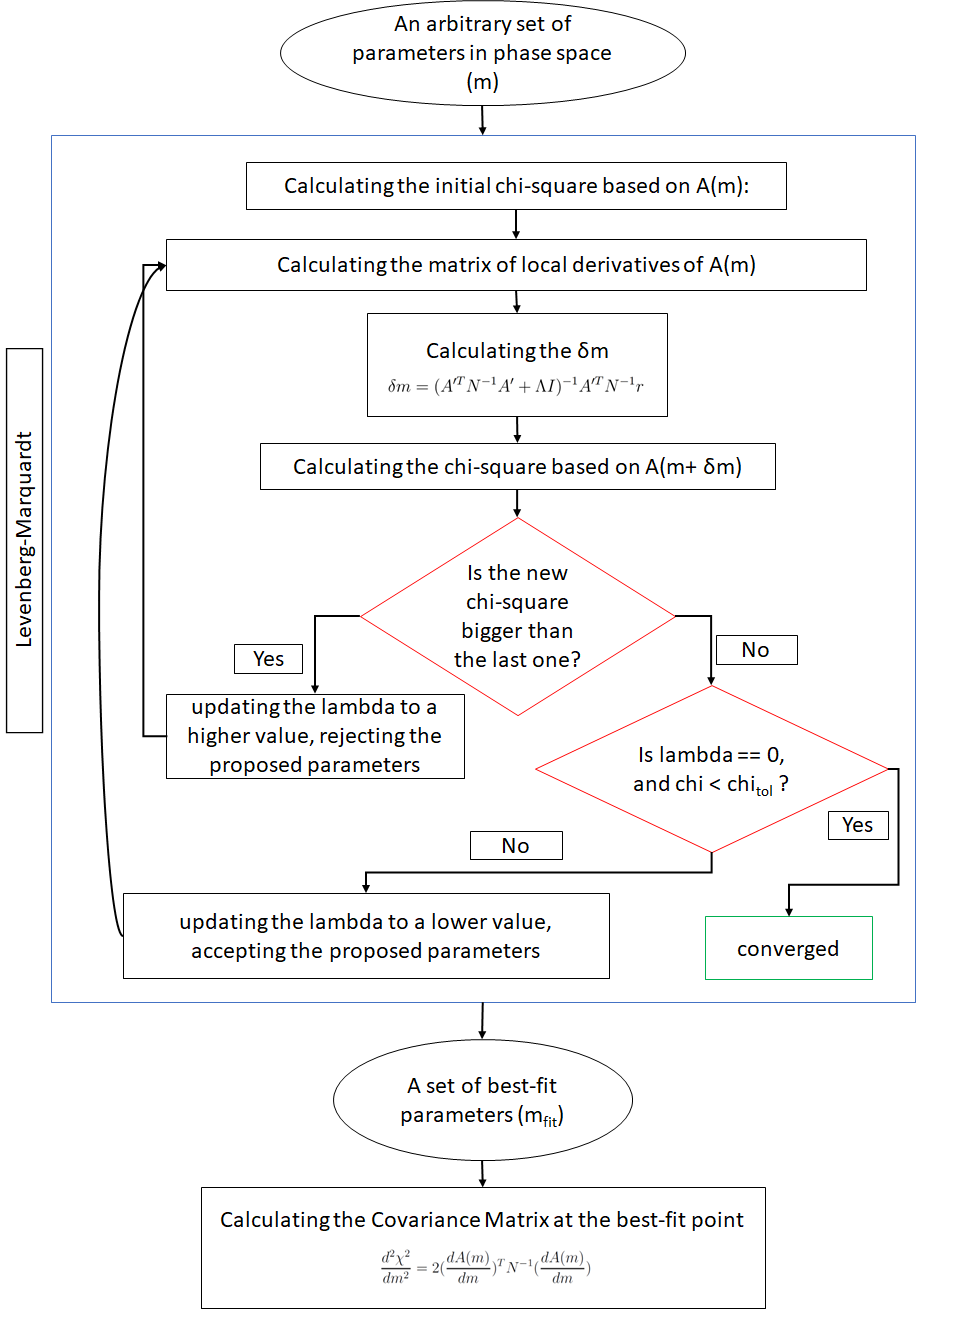
\includegraphics[scale =0.9]{LM_flow.png}
\caption{Flow chart of Levenberg-Marquardt algorithm}
\label{fig:LM_flow}
\end{figure}
%--------------------------------------------------------------------------------
\section{Markov Chain Monte Carlo (MCMC)}
Given that Levenberg-Marquardt (LM) is not always effective in finding the best-fit point for complex likelihood spaces, a more powerful algorithm such as Markov Chain Monte Carlo (MCMC) is necessary in many real-life applications. \par
MCMC is particularly effective in fitting non-Gaussian likelihood spaces and has a guaranteed convergence, regardless of the starting point in parameter space. However, the algorithm is computationally heavy due to its iterative process, which is based on the evaluation of chi-square on each step. Initially, an arbitrary point in parameter space is given to MCMC as its initial trial step and the associated chi-square is calculated. Then, a random point is drawn from a Gaussian distribution, where the mean is set at the last point in the chain \footnote{In Python applications, the numpy.randn function is used to serve this purpose.}. Subsequently, the new chi-square is compared to the previous one from the last trial step. If the new chi-square is lower, the new trial point is accepted in the chain. If the new chi-square is higher, the trial point is accepted with a probability determined by a specific criterion.\par
The above-mentioned probability threshold is typically defined as:
\begin{equation}
    Probability = e^{\frac{-1}{2}(\chi_{new}^2 - \chi^2)}
\end{equation}
Which again has Gaussian insights.\par
As a measure of MCMC performance, the acceptance ratio is used to determine the fraction of trial steps that end up getting accepted into the chain. An ideal MCMC would typically have an acceptance ratio of 25 percent. However, even with a lower acceptance ratio, the MCMC can still converge, but it will require more trial steps.\par
A visual summary of MCMC algorithm is shown in \ref{fig:MCMC_flow}, and the Python code is available at \ref{chap:appendix,sub:MCMC}.
\begin{figure}[h!]
\centering
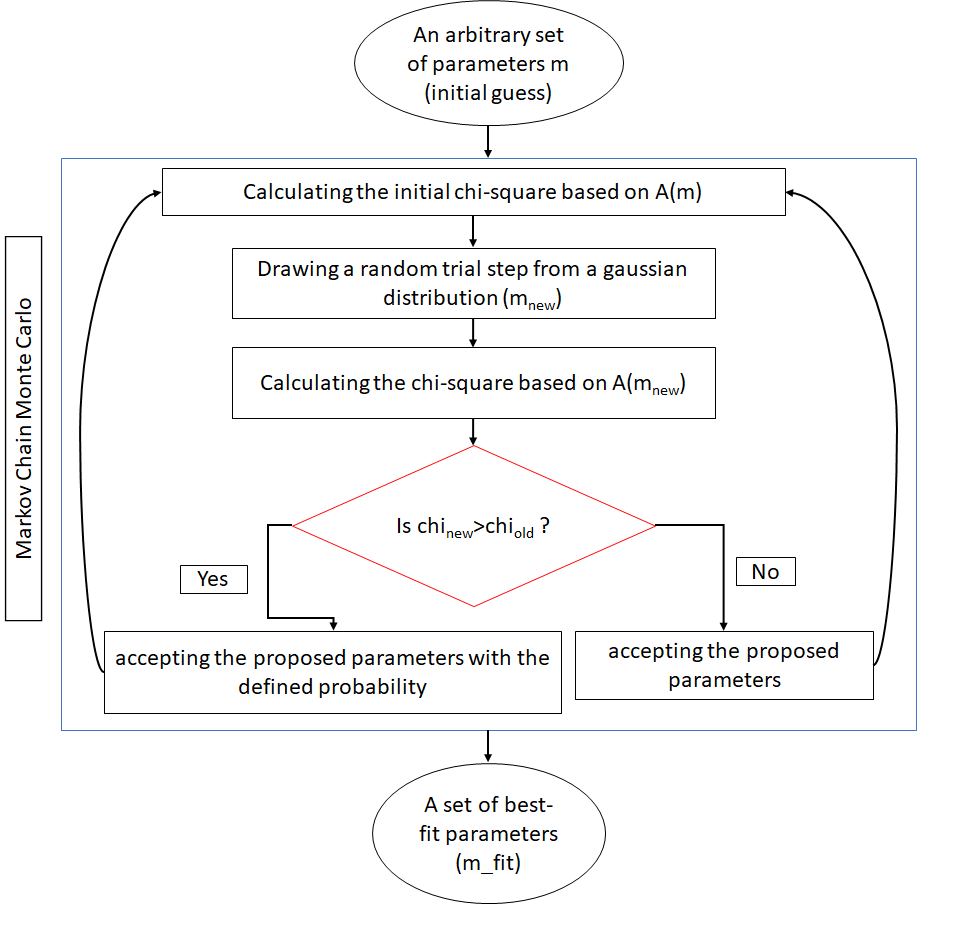
\includegraphics[scale =0.9]{MCMC_flow.png}
\caption{Flow chart of MCMC algorithm}
\label{fig:MCMC_flow}
\end{figure}
%-----------------------------------------------------------------------------
\subsection{Convergence Test}
The MCMC algorithm is designed to explore different regions of the parameter space in order to reach convergence. Various methods have been developed to ensure that the MCMC has converged, one of which is to check the power spectrum.\par
The power spectrum represents the distribution of power at different frequencies in the MCMC chain. A converged MCMC chain must have the behaviour of a white noise, with power uniformly distributed among all frequencies. On the other hand, an unconverged chain will show more power at lower frequencies compared to higher ones. Therefore, the criterion for checking the convergence of an MCMC chain is the flatness of the power spectrum in low frequencies when plotted on a log-log scale. Figure \ref{fig:MCMC_unconverged} and \ref{fig:MCMC_converged} illustrates the difference between a converged and an unconverged chain.\par
\begin{figure}[h!]
\centering
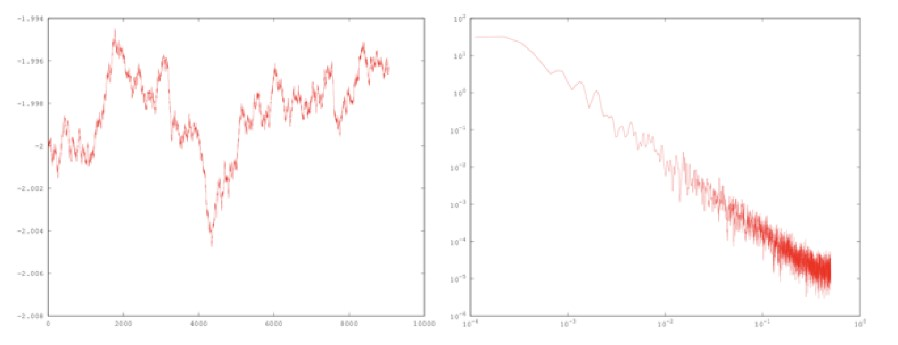
\includegraphics[scale =0.9]{mcmc_uncoverged.jpg}
\caption[An unconverged MCMC chain and its power spectrum]{An unconverged MCMC chain (left panel) and its power spectrum (right panel): The power tend to increase in lower frequencies, the chain itself does not indicate the behaviour of white noise, plot from Jonathan Sievers}
\label{fig:MCMC_unconverged}
\end{figure}

\begin{figure}[h!]
\centering
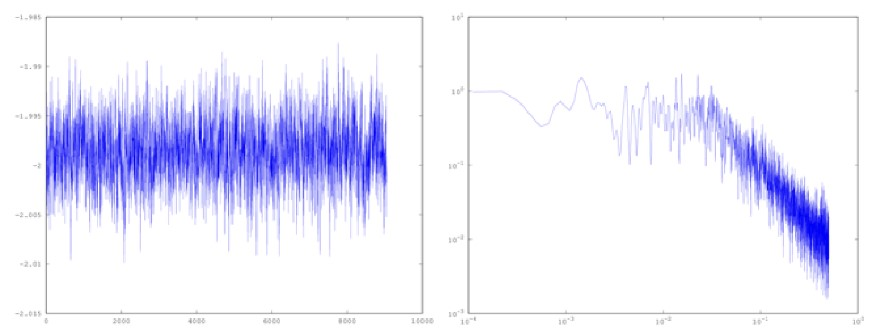
\includegraphics[scale =0.9]{mcmc_converged.jpg}
\caption[A converged MCMC chain and its power spectrum]{A converged MCMC chain (left panel) and its power spectrum (right panel): Note the flatness on low frequencies, plot from Jonathan Sievers}
\label{fig:MCMC_converged}
\end{figure}
%------------------------------------------------------------------------------------------------------
\section{Combination of MCMC and LM}
As mentioned before, MCMC is a computationally heavy algorithm due to its iterative nature. If calculating the chi-square takes a long time on each step, the MCMC itself will have a rather long run time before reaching the converged state. Different methods have been proposed to deal with this issue and help the MCMC to converge faster, one of which is to use the insights from running LM.\par
We previously discussed that parameters of a model might be correlated (\ref{chap:method,sub:cov_mat}). During a simple MCMC, we are drawing random samples from a gaussian distribution. This samples do not take the possible correlations into account. However, if we generate samples with such characteristics, the probability of them getting accepted into the actual chain is higher. Therefore, this approach (feeding the MCMC with a posterior distribution) will eventually assist the MCMC to explore more efficient regions of parameter space, and converge faster. Figure \ref{fig:combined_flow} illustrates this technique briefly.\par
Since the covariance matrix of these needed samples is already in hand, we are able to easily generate a set of correlated noise samples from that. This procedure is described in the following section.\par

\begin{figure}[h!]
\centering
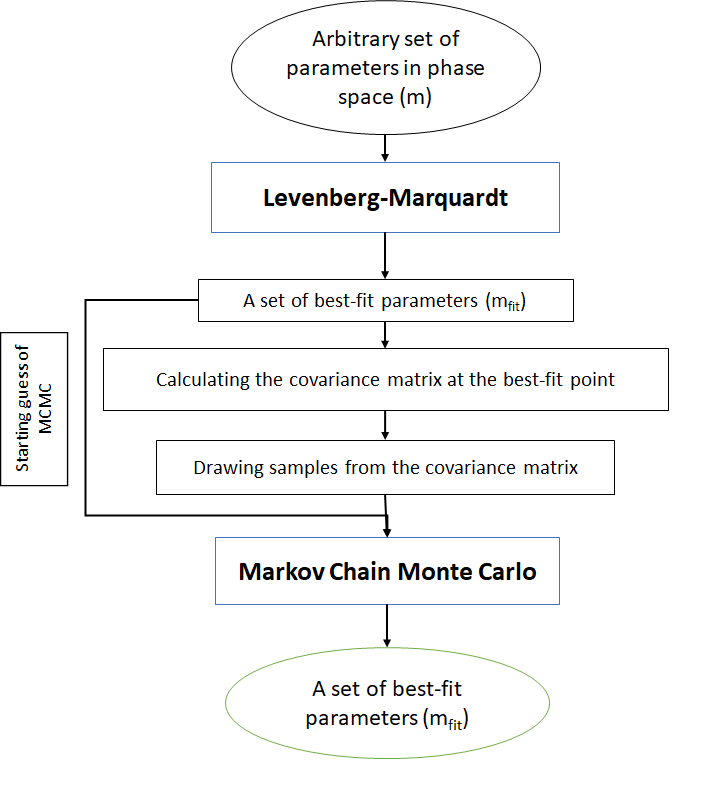
\includegraphics[scale =0.9]{combined_flow.png}
\caption{Flow chart of the procedure to combine MCMC and LM}
\label{fig:combined_flow}
\end{figure}

\subsection{Generating correlated noise}
\label{chap:method,sub:correlated noise}
As discussed before, the off-diagonal elements of a covariance matrix correspond to the inverse of covariance between each pair of parameters. Thus, if we draw samples from the inverse of covariance matrix (which needs to be calculated at the point of "best-fit"), we are essentially sampling from the multivariate normal distribution with the deviation values describing the uncertainties in the parameters\footnote{Figure \ref{fig:corner_plots}, which shows the corner plots for a four-variable gaussian model, emphasizes the importance of sampling from a multivariate normal distribution and taking the correlations between the parameters into account.}.\par
The equivalent methods can be used to generate correlated noise: Cholesky and eigenvalue decomposition\footnote{Normally, calculating the Cholesky decomposition takes a shorter amount of time.}. For practical reasons, we prefer to use the eigenvalue decomposition for 21cm applications. The procedure is a s follows: A matrix of normal gaussian-drawn random variables is constructed in the desired shape ($n \times m$, corresponding to the number of samples and number of parameters respectively). Then, it is multiplied by the eigenvalue matrix and scaled by the square root of the eigenvalues. The transpose of the product will give us the correlated samples. \par
To gain more precision, is it possible to use the eigenvalues decomposition of the normalized covariance matrix (where diagonal samples all equal unity). The normalization process is done by multiplying the covariance matrix with its own diagonal. Eventually, the drawn samples need to be scaled by the square root of the diagonal matrix.\par
The Python implementation of the above-mentioned procedure is given in \ref{chap:appendix,sub:draw}.

\begin{figure}[h!]
\centering
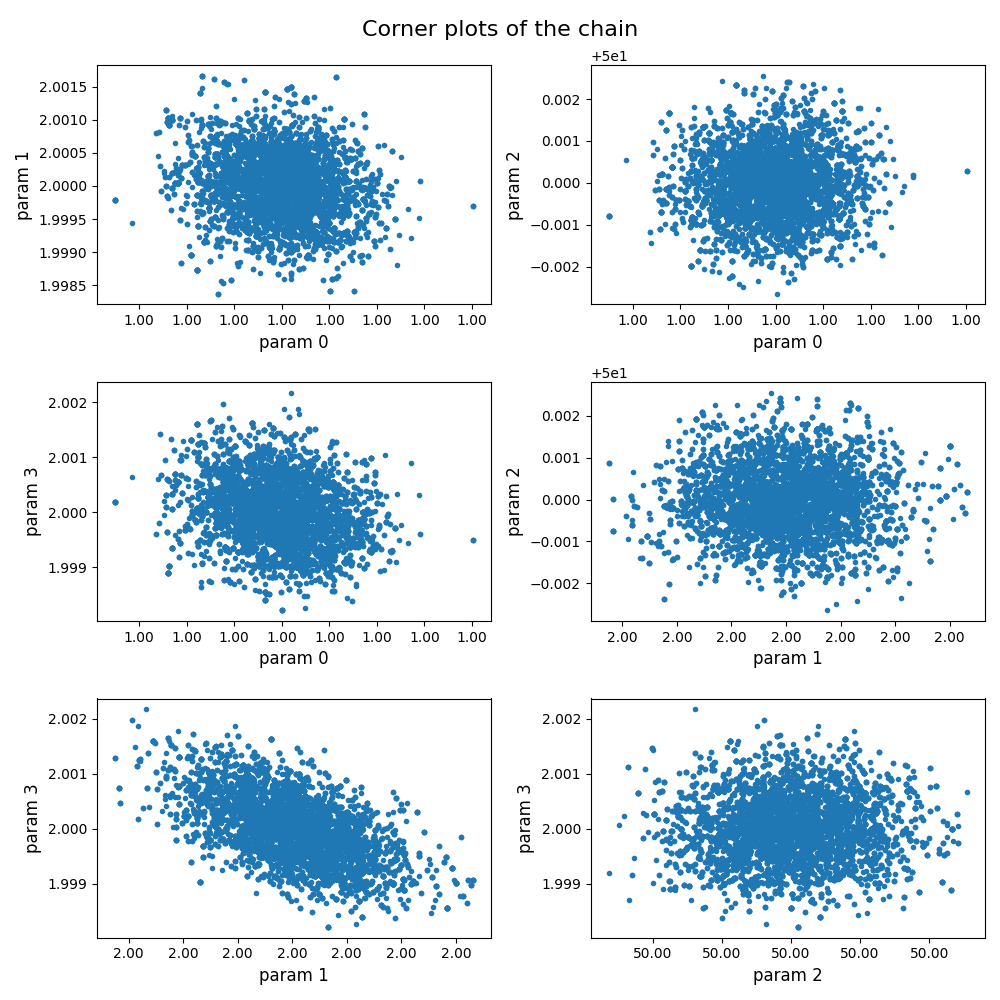
\includegraphics[scale =0.6]{corner_plot_chain.png}
\caption[Corner plots of an MCMC chain]{Corner plots (parameter vs parameter) of a typical MCMC chain imposed on a four-variable gaussian model. The lower right panel clearly shows patterns of correlation between a pair of parameters. Sampling from a multivariate normal distribution based on the covariance matrix of these samples helps taking the correlations between these parameters into account.}
\label{fig:corner_plots}
\end{figure}

\section{Testing the Algorithm}
The complicated algorithm described in the previous sections, does not always behave as expected. Thus, naturally, one seeks options to weigh the output. In sections \ref{chap:method,sub:test,subsub:chi} and \ref{chap:method,sub:test,subsub:plot}, we introduce two methods to measure the overall quality of the model fitting.\par
\subsection{The chi-square test}
\label{chap:method,sub:test,subsub:chi}
This method is more focused on inspecting the output of LM and drawn samples. A large number of samples are drawn from the covariance matrix and the corresponding chi-squares are calculated. Since the covariance matrix describes the uncertainties in the parameters, we expect that the average difference in the chi-square statistics for two different samples should be of order unity per each parameter. This comes from the fact that the chi-square statistic scales with the uncertainties in the data and model, which are typically of order 1.\par
Figure \ref{fig:csq_test} shows an example of the distribution of difference between the chi-square values.\par
\begin{figure}[h!]
\centering
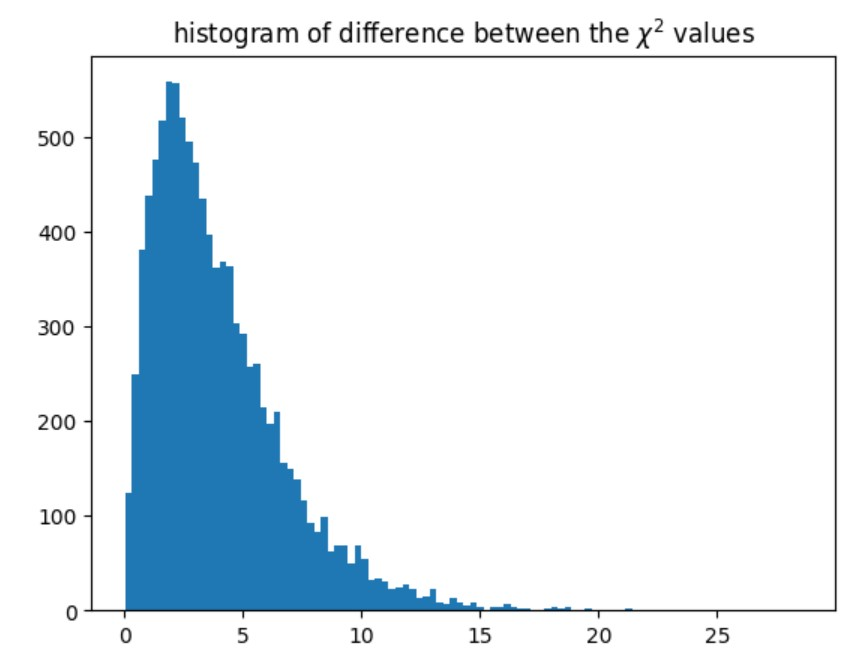
\includegraphics[scale =0.9]{chi-sqaure test.jpg}
\caption[Histogram of difference in the chi-square values of drawn samples]{Histogram illustrating the distribution of the values of difference between the chi-squares of drawn samples for a four variable model. The average is 3.97 and the standard deviation is 2.83, in agreement with our expectations. The best-fit parameters is considered as a "good fit".}
\label{fig:csq_test}
\end{figure}
\subsection{Chi-Square vs Parameters Plots}
\label{chap:method,sub:test,subsub:plot}
Another method to verify the results is to plot the chi-square values of drawn samples versus the each of the parameters. According to the definition of chi-square \ref{eq:chi-square matrix} (the non-linear dependency of chi-square on model parameters) we expect to observe a parabolic behaviour.\par
Figure \ref{fig:csq_params} demonstrates chi-square vs parameters plots for the same model as \ref{fig:csq_test}.
\begin{figure}[h!]
\centering
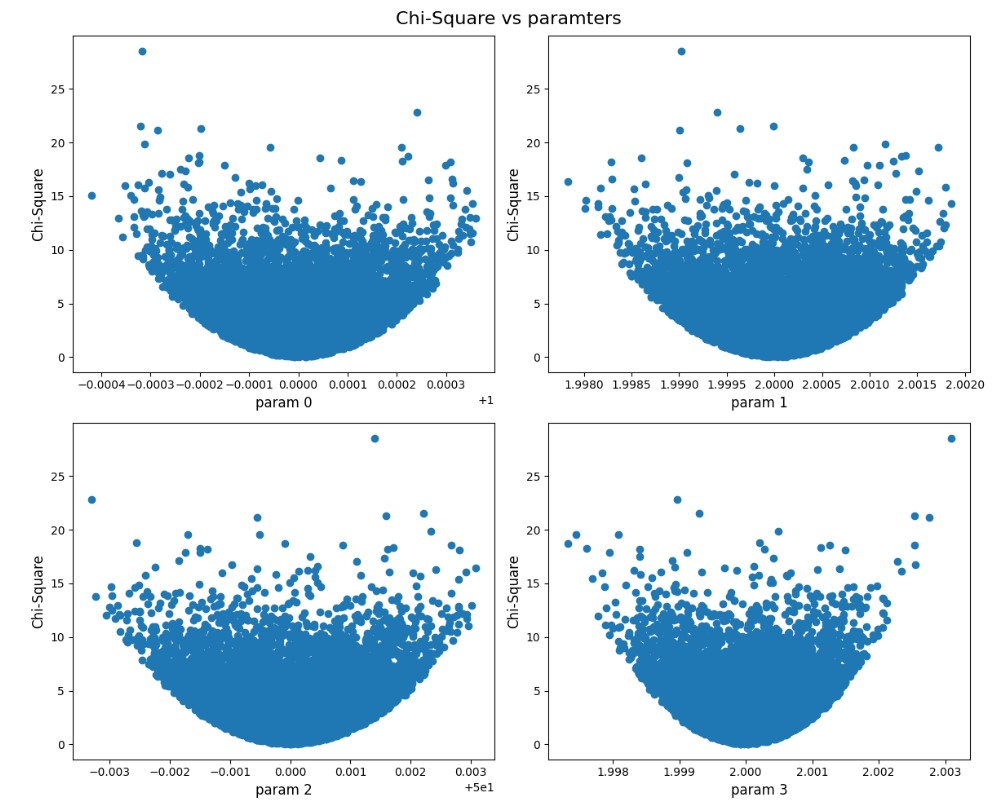
\includegraphics[scale =0.9]{csq_params.jpg}
\caption[Chi-Square vs parameters plots]{Plots of the values of chi-square of drawn samples versus the values of parameters for a four variable model. The parabolic behaviour is obvious.}
\label{fig:csq_params}
\end{figure}
%###################################################################################
\chapter{Results and Analysis}
\label{chap:results}
Reminder: citations for physical explanation of parameters\par
Chapter \ref{chap:method} carefully described a specific method to fit an experimental data set to its corresponding theoretical model. In this chapter, we are going to impose this method to actual global 21cm curves. We chose to use ARES as our simulator to generate these curves. \par
As discussed in chapter \ref{chap:global21cm}, the physical model of 21cm curve is dependent on a large number of parameters. However, this model can be effectively described using the following parameters:
\begin{enumerate}
    \item \textbf{$N_{lw}$}: Number of photons emitted in the Lyman-Werner band ($11.2-13.6eV$) per baryon of star formation (This parameter is referred to as \emph{pop\_rad\_yield\_0\_} in ARES documentation)
    \item \textbf{$N_{ion}$}: Mean number of ionizing photons produced per baryon of star formation (This parameter is referred to as \emph{pop\_rad\_yield\_2\_} in ARES documentation)
    \item \textbf{$f_{esc}$}: Fraction of ionizing photons that escape their host galaxy into the IGM
    \item \textbf{$f_X$}: High-redshift normalization factor in the relation between X-ray luminosity and SFR
\end{enumerate}
Figure \ref{fig:sensivity} shows the effect of changing these parameters on an actual 21cm curve.\par

\begin{figure}[h!]
\centering
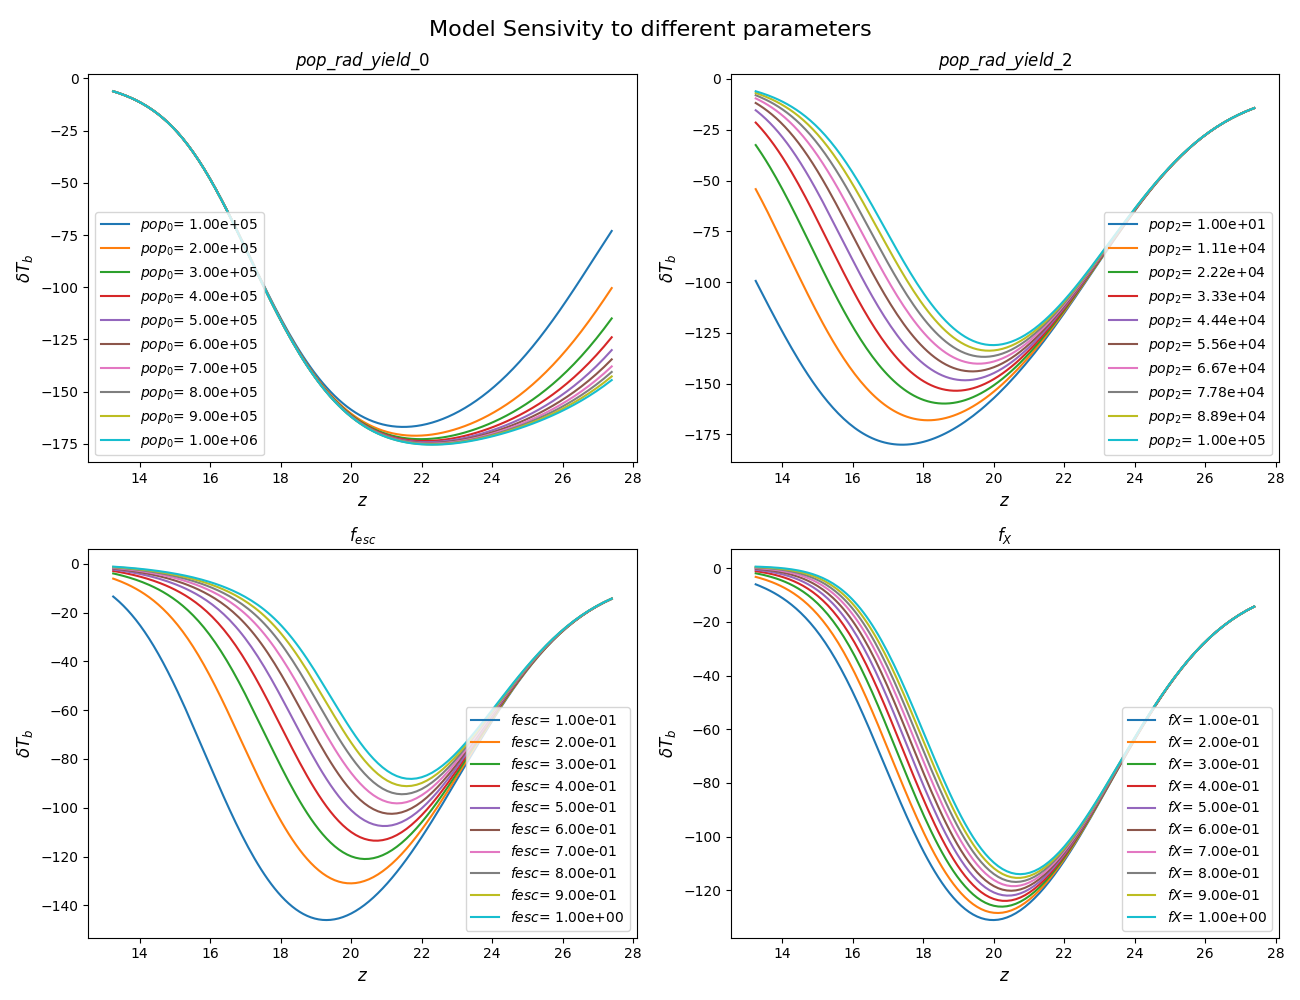
\includegraphics[scale =0.6]{sensivity.png}
\caption[Behaviour of global 21cm model in reaction to change in four parameter]{Behaviour of ARES-generated global 21cm models with respect to four parameters: \emph{pop\_rad\_yield\_0\_}, \emph{pop\_rad\_yield\_2\_}, $f_{esc}$, and $f_X$. In each panel, the corresponding parameter posses 10 different values and all other parameters are kept at default values by ARES}
\label{fig:sensivity}
\end{figure}
We take the above-mentioned physical parameters as fitting parameters and we try to find their best-fit values and corresponding error-bars.\par
%-----------------------------------------------------------------------------------
\section{Parameter Estimation of an ARES generated curve}
Before using our developed script to fit actual data, we use it to fit a known ARES curve as a verification test. We generate an ARES curve with a fixed set of parameters and we use these curve as the imaginary "data". If the algorithm returns the same parameter values (with in the error-bar range), we can make sure that it is working correctly.\par
We begin by using the LM and we find inverse of covariance matrix for our chosen combination of parameters:\par
Parameters:
\begin{equation}
\emph{pop\_rad\_yield\_0\_}: 10^4, \quad \emph{pop\_rad\_yield\_2\_}: 10^3,\quad f_{esc}: 0.1,\quad f_X: 0.1 
\end{equation}
Inverse of covariance matrix for this set of parameters:
\begin{equation}
    \begin{pmatrix}
    1.64\times 10^{-3} & 1.96 \times 10^{-2} &  -4.39 \times 10^{-7} &  -5.37 \times 10^{-8} \\
    1.96 \times 10^{-2} &  1.60 \times 10^{1} &  -1.44 \times 10^{-3} &  -5.94 \times 10^{-6} \\
    -4.39 \times 10^{-7} &  -1.44 \times 10^{-3} &  1.38 \times 10^{-7} &  2.15 \times 10^{-10} \\
    -5.37 \times 10^{-8} &  -5.94 \times 10^{-6} &  2.15 \times 10^{-10} &  1.38 \times 10^{-11} 
    \end{pmatrix}
\end{equation}
\begin{figure}[h!]
\centering
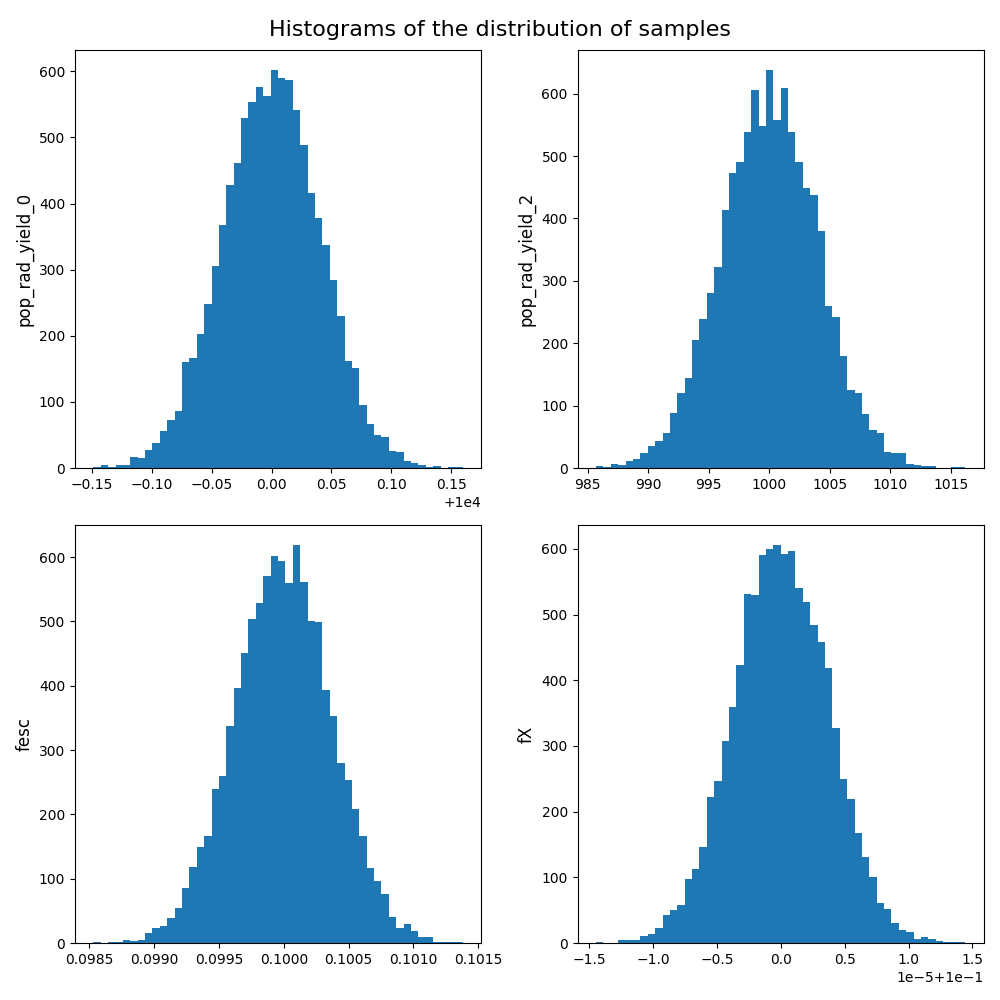
\includegraphics[scale =0.6]{histograms_known_curve.png}
\caption[Histogram of distribution of samples]{Histogram of distribution of samples before feeding to MCMC}
\label{fig:histogram_samples_known_curve}
\end{figure}

\begin{figure}[h!]
\centering
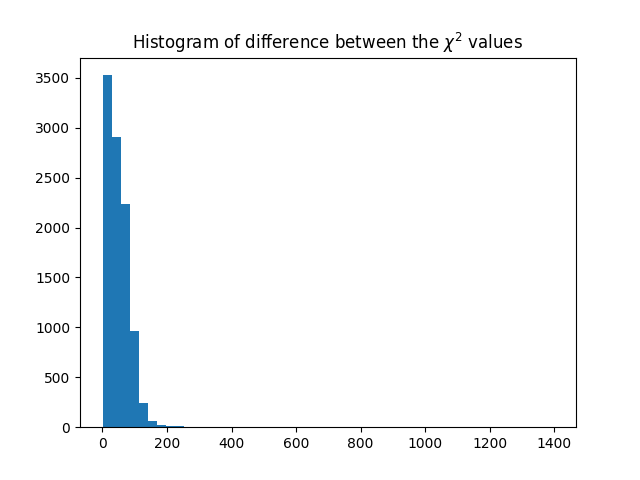
\includegraphics[scale =0.9]{csq_hist_known_curve.png}
\caption[Histogram of Chi-Square of drawn samples]{Histogram of Chi-Square of drawn samples}
\label{fig:csq_hist_known_curve}
\end{figure}

\begin{figure}[h!]
\centering
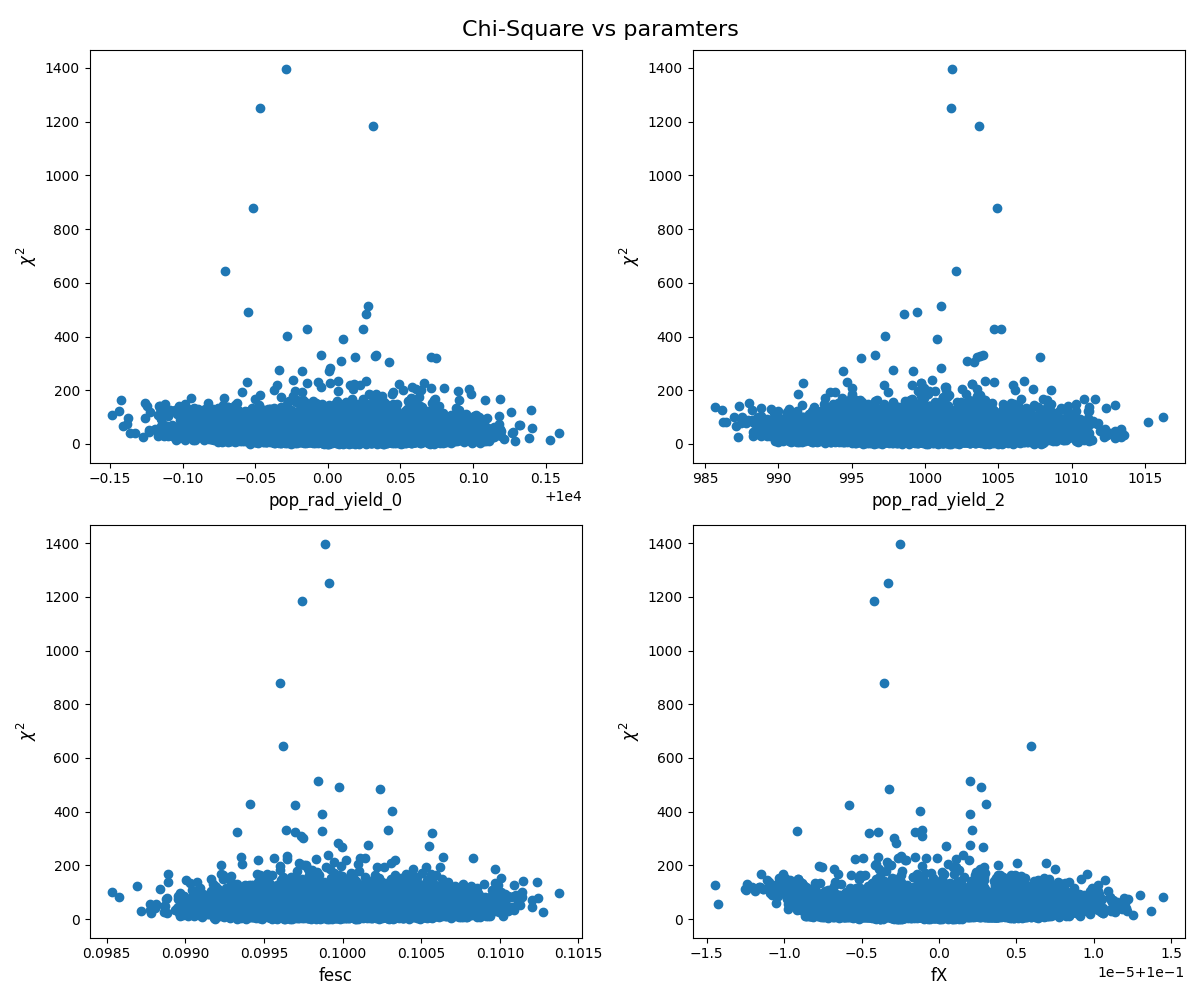
\includegraphics[scale =0.5]{csq_vs_params_knwon_curve.png}
\caption[Chi-Square of Drawn samples vs parameter values]{Chi-Square of Drawn samples vs parameter values}
\label{fig:csq_vs_params_knwon_curve}
\end{figure}

\begin{figure}[h!]
\centering
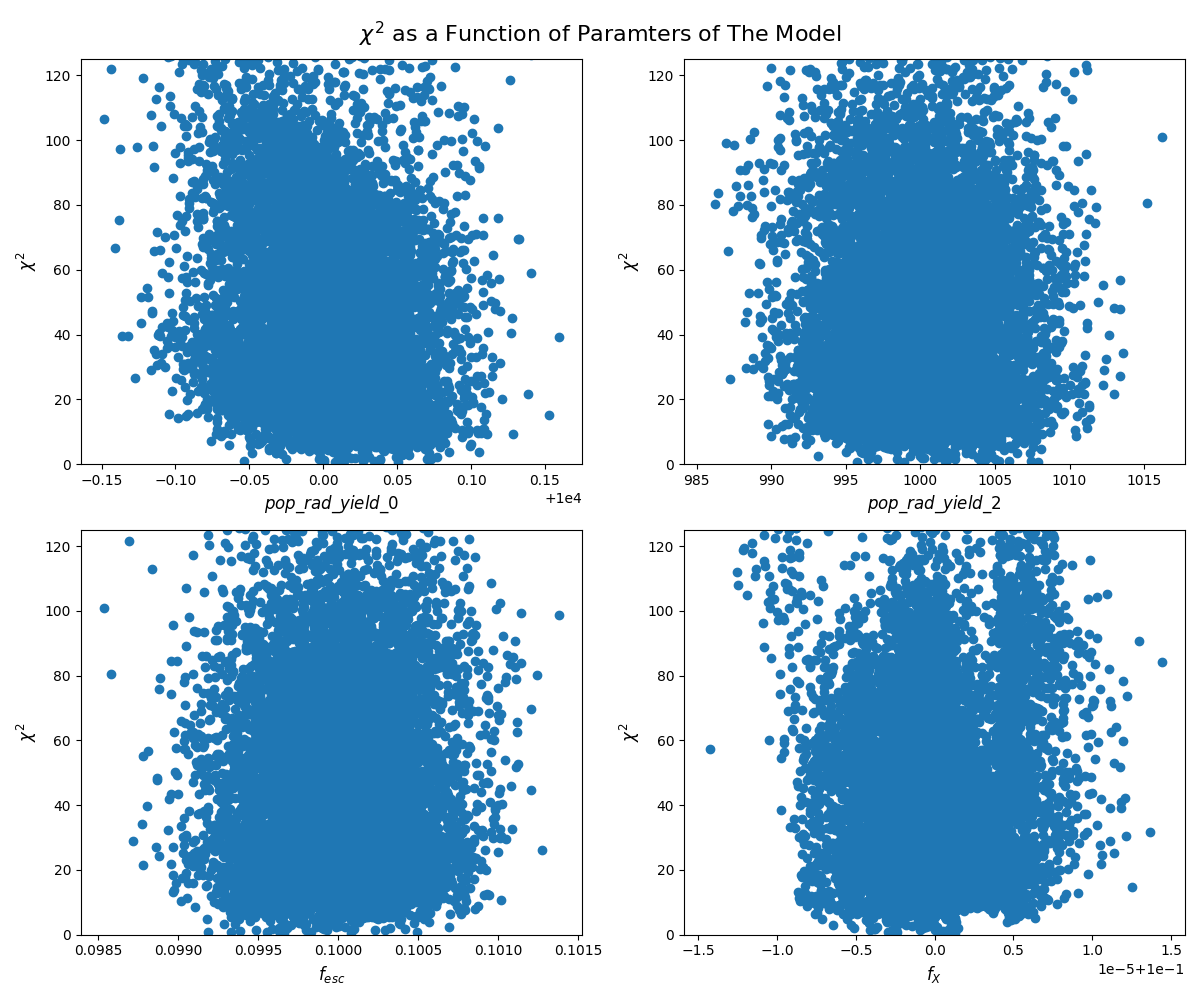
\includegraphics[scale =0.5]{csq_vs_params_zoomed_known_curve.png}
\caption[Chi-Square of Drawn samples vs parameter values, zoomed]{Chi-Square of Drawn samples vs parameter values, zoomed}
\label{fig:csq_vs_params_zoomed_known_curve}
\end{figure}

\begin{figure}[h!]
\centering
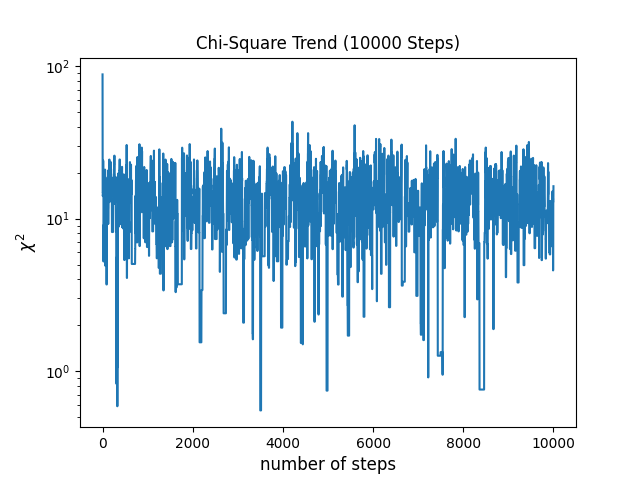
\includegraphics[scale =0.9]{csq_trend_knwon_curve.png}
\caption[Trend of chi-square]{Trend of chi-square}
\label{fig:csq_trend_knwon_curve}
\end{figure}

\begin{figure}[h!]
\centering
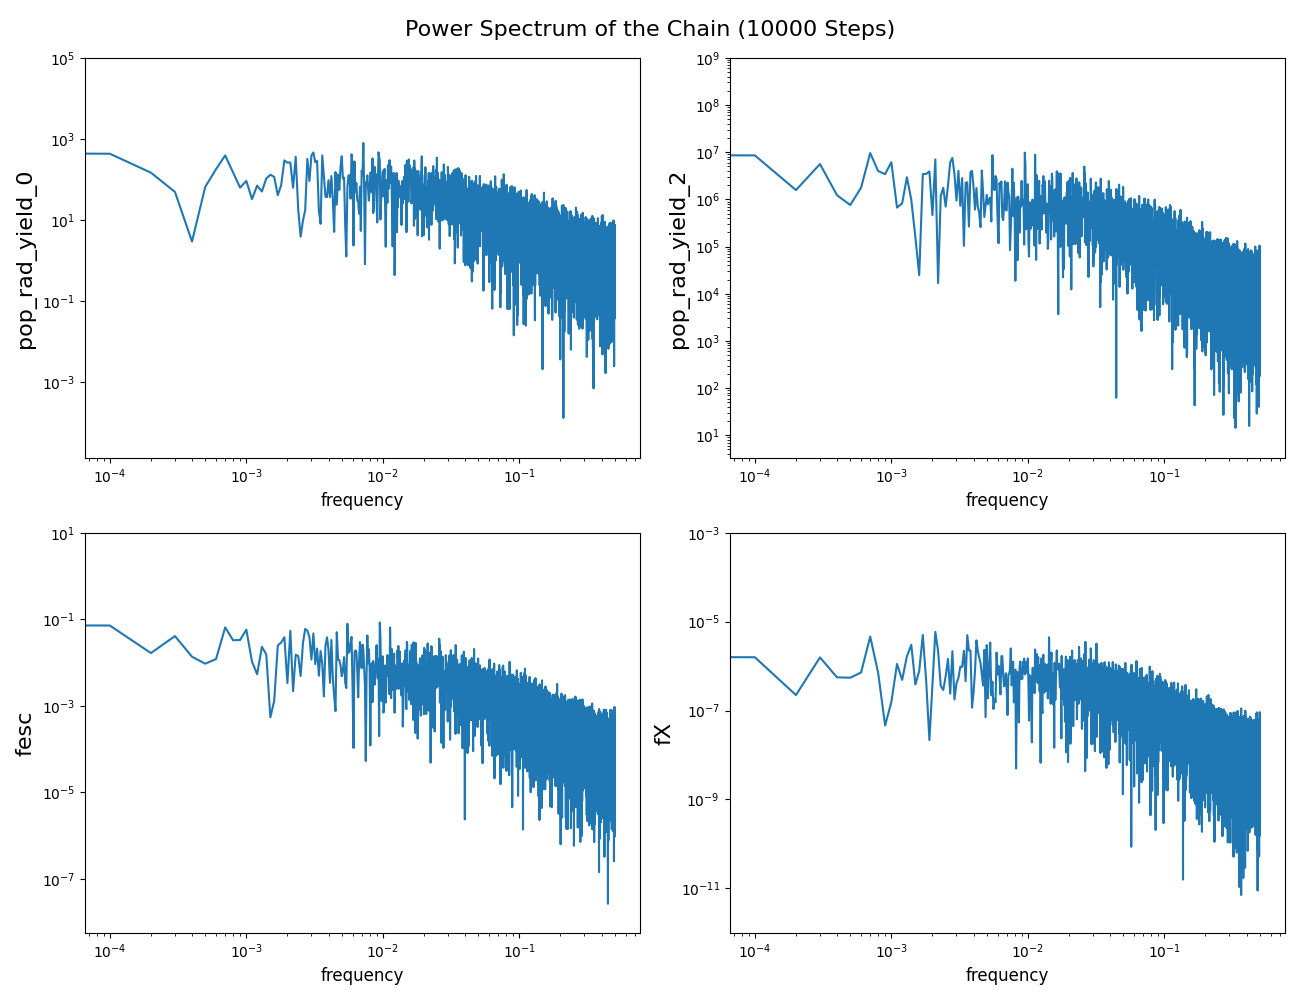
\includegraphics[scale =0.5]{power_spectrum_known_curve.png}
\caption[Power spectrum of the chain]{Power spectrum of the chain}
\label{fig:power_spectrum_known_curve}
\end{figure}

\begin{figure}[h!]
\centering
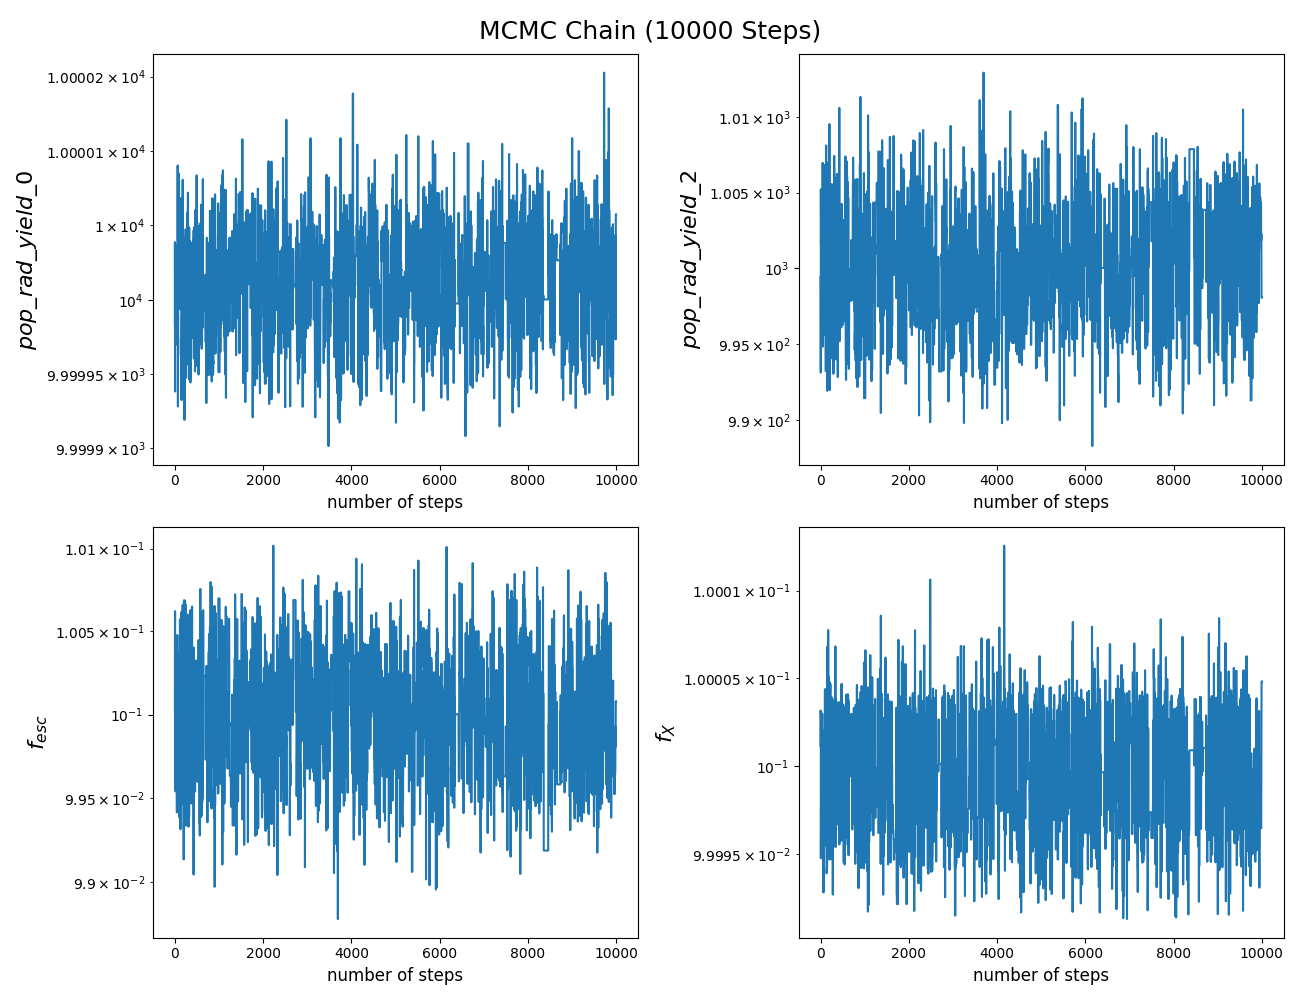
\includegraphics[scale =0.5]{chain_known_curve.png}
\caption[Trend of parameters]{Trend of parameters}
\label{fig:chain_known_curve}
\end{figure}

\begin{figure}[h!]
\centering
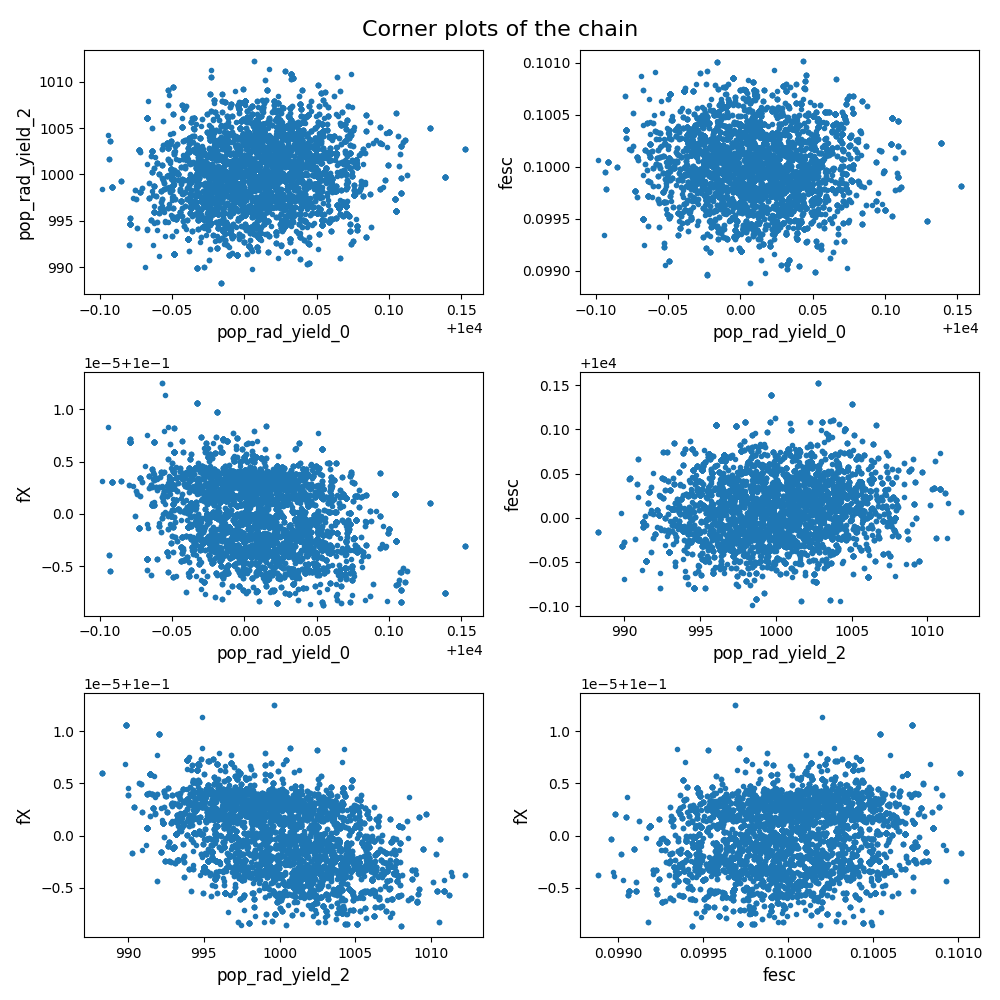
\includegraphics[scale =0.6]{corner_plots_known_curve.png}
\caption[Corner plots of the chain]{Corner plots of the chain}
\label{fig:corner_plots_known_curve}
\end{figure}
%------------------------------------------------------------
\section{Choice of "multiplication factor"}
%-----------------------------------------------------------------------------------
\section{Parameter estimates of EDGES data and uncertainties}
\subsection{error bar calculation}
%-----------------------------------------------------------------------------------
\section{Comparison with previous studies and observations}
I will write this section after the literature review
%###################################################################################
\chapter{Discussion and Conclusion}
\label{chap:discussion}
\section{Interpretation of the results}
%\section{Implications for cosmology and astrophysics}
\section{Summary of the main findings}
\section{Contributions and significance of the research}
\section{Limitations and future work}
%##############################################################################
\chapter{Appendices}
\section{Code snippets and scripts}	
\subsection{Levenberg-Marquardt}
\label{chap:appendix,sub:LM}
\subsection{Markov Chain Monte Carlo}
\label{chap:appendix,sub:MCMC}
\subsection{drawing samples from covariance matrix}
\label{chap:appendix,sub:draw}
\begin{lstlisting}[language=Python, caption=Python example]
    def draw_samples(covariance_matrix, nset):
    """
    covariance_matrix: covariance matrix
    nset:the number of samples
    returns: a matrix of samples
    This function calculates a series of correlated samples based on the presented 
    covariance matrix and the number of samples.
    The shape of the output is (nset, m) where m comes from the shape of 
    covariance matrix and it typically shows the number of parameters in the model.
    """
    #normalizing the covariance matrix
    D = np.diag(np.diag(covariance_matrix)) #diagonal matrix of covariance matrix
    D_sqrt = np.sqrt(D)
    D_inv_sqrt = np.linalg.pinv(D_sqrt)
    #normalized covariance matrix
    covariance_matrix_normalized = D_inv_sqrt @ covariance_matrix @ D_inv_sqrt 

    e,v = np.linalg.eigh(covariance_matrix_normalized)
    e[e<0]=0 #omitting any negative eigenvalues due to roundoff
    n = len(e)

    #make gaussian random variables
    g=np.random.randn(n, nset)

    #scaling by the square root of the eigenvalues
    rte=np.sqrt(e)
    for i in range(nset):
        g[:,i]=g[:,i]*rte

    #calculating the samples
    samples = (v@g).T
    #denormalizing the samples
    samples_denormalized = samples @ D_sqrt
    return samples_denormalized
\end{lstlisting}
	% Begin Bibliography
	{
	
	\bibliography{references}
	\bibliographystyle{ieeetr}
	
	}
\end{document}